\documentclass[10pt,a4paper]{article}
\usepackage[utf8]{inputenc}
\usepackage{amsmath}
\usepackage{amsfonts}
\usepackage{amssymb}
\usepackage{palatino}
\usepackage[left=3cm,right=3cm,top=3cm,bottom=3cm]{geometry}
\usepackage{geometry}
\usepackage{listings}
\usepackage{amsmath,amsthm}
\usepackage{extpfeil}
\usepackage{indentfirst}
\usepackage{mathptmx}
\usepackage{subfig}
\usepackage{graphicx}
\usepackage{diagbox}
\usepackage{cite}
\global\long\def\d{\text{d}}
\newtheorem{proposition}{Proposition}
\newtheorem{definition}{Definition}
\newtheorem{corollary}{Corollary}
\newtheorem{claim}{Claim}
\newtheorem{theorem}{Theorem}
\newtheorem{lemma}{Lemma}
\newtheorem{fact}{Fact}
%\usepackage{booktabs}
%\usepackage{lipsum}
\title{DSGA-1011 Natural Language Processing with Representation Learning Homework 1
}
\author{Xintian Han (xh1007)}
\begin{document}
\maketitle
\section{Bag of N-Gram Document Classification} 
We build a bag of n-grams model for predicting the sentiment of the movie reviewers given the textual review for the movie. We use IMDB review dataset consisting of 25,000 train and 25,000 test movie reviews scraped from IMDB website. We split the train dataset into 20,000 train examples and 5,000 validation examples. We perform the hyperparameter tuning on the validation set and report the result of the best model on the test set. We use the following set of hyperparameters.
\begin{itemize}
\item Tokenization schemes of the dataset: 
\begin{itemize}
\item 'en\_core\_web\_sm'	
\end{itemize}
\item Model hyperparameters:
\begin{itemize}
\item Vary n for n-gram (n=1, 2, 3, 4)
\item vocabulary size (5000, 10000, 20000)
\item embedding size (100, 200, 500)
\end{itemize}
\item Optimization hyperparameters:
\begin{itemize}
\item Optimizer itself (SGD vs Adam)
\item Learning rate [0.1, 0.01, 0.001]
\item Whether or not you use linear annealing of learning rate (learning rate is reduced linearly over the course of training).	
\end{itemize}
\end{itemize}
For n-grams, there are two strategies. One is using only n-gram; the other is using all the k-gram until n, i.e. 4-grams including 1,2,3,4-grams. We consider both two strategies. So there are 7 choices of n-grams. There are total $7\times 3 \times 3\times 2 \times 3 \times 2 = 756$ different combinations. We first perform the ablation study. We also did an enumerative study but it took too long time and did not finish in two days. We keep the partial results of learning curves and training output in the folder and the notebook $\texttt{enumerative\_search.iynb}$. Unfortunately, we could not finish the enumerative search. The main work in this report is based on ablation study in $\texttt{hw1.ipynb}$.
\subsection{Vary Vocabulary Size and Embedding Size,  and Fix the Others}
We use n-gram = unigram, Adam, fixed-learning rate = 0.001, test vocabulary size and embedding size.
The accuracy on the validation set is shown in Table \ref{tab: vocab_emb}.
\begin{table}[!ht]
\centering
\begin{tabular}{|l|c|c|c|}
\hline
Accuracy& 	vocab\_size = 5000 & vocab\_size = 10000 &vocab\_size = 20000 \\ \hline
emd\_size = 100& 83.2 & 83.04 & 82.94\\ \hline
emd\_size = 200 & 83.56 & 82.78 & 82.48\\ \hline
emd\_size = 500 & 82.8 & 81.54 & 81.54 \\ \hline
\end{tabular}
\caption{\label{tab: vocab_emb} Accuracy on Validation Set When We Vary Vocabulary Size and Embedding Size,  and Fix the Others.}
\end{table}
\begin{figure}[!ht]
\centering
\subfloat[(5000,100)]{
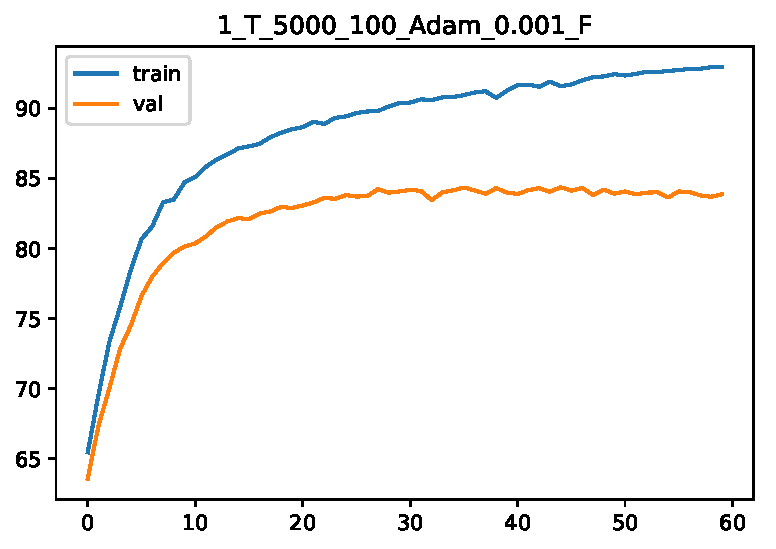
\includegraphics[width = 3cm]{1_T_5000_100_Adam_0001_F.pdf}
}
\subfloat[(10000,100)]{
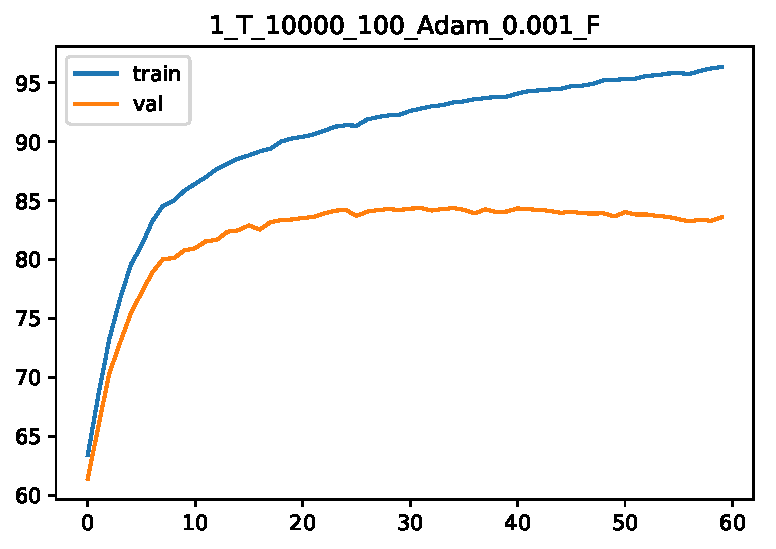
\includegraphics[width = 3cm]{1_T_10000_100_Adam_0001_F.pdf}
}	
\subfloat[(20000,100)]{
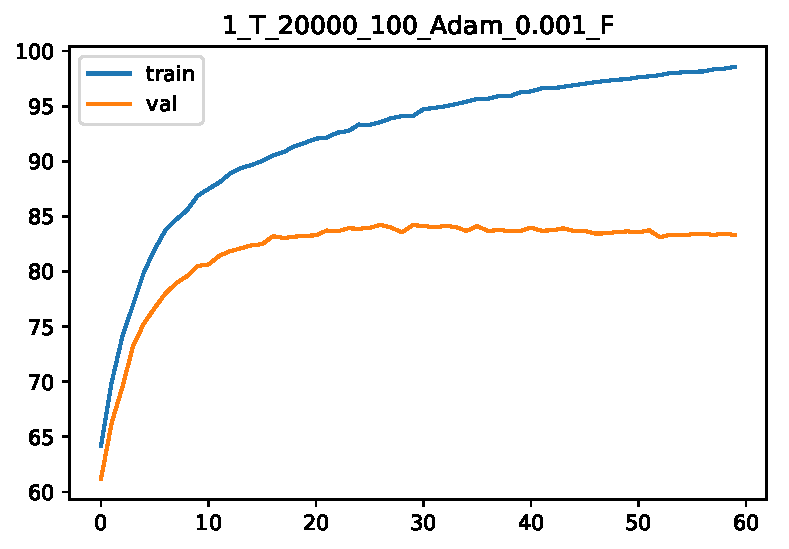
\includegraphics[width = 3cm]{1_T_20000_100_Adam_0001_F.pdf}
}
\subfloat[(5000,200)]{
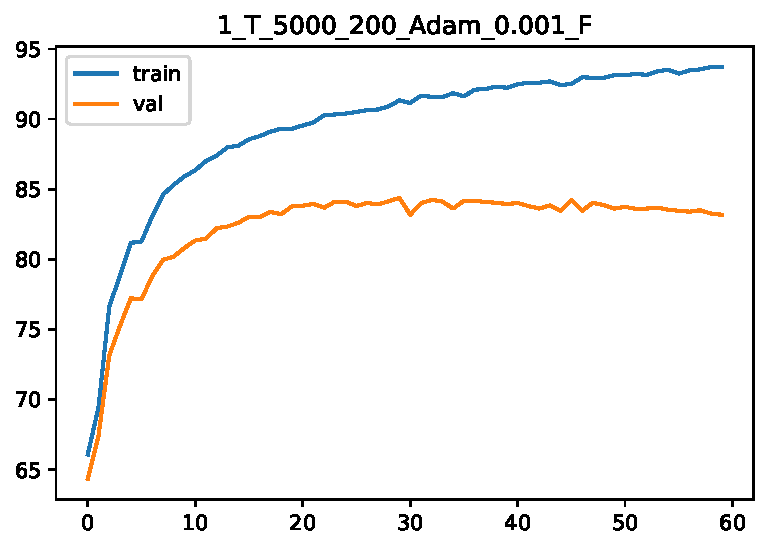
\includegraphics[width = 3cm]{1_T_5000_200_Adam_0001_F.pdf}
}		
\subfloat[(10000,200)]{
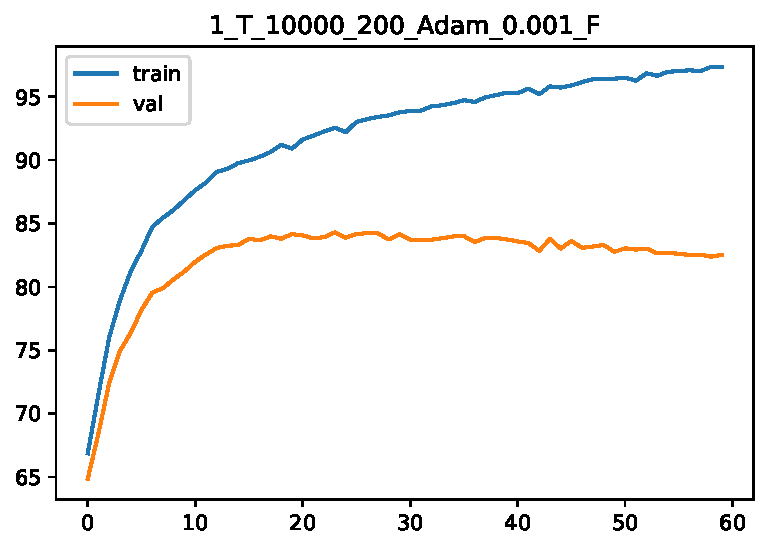
\includegraphics[width = 3cm]{1_T_10000_200_Adam_0001_F.pdf}
}	\\
\subfloat[(20000,200)]{
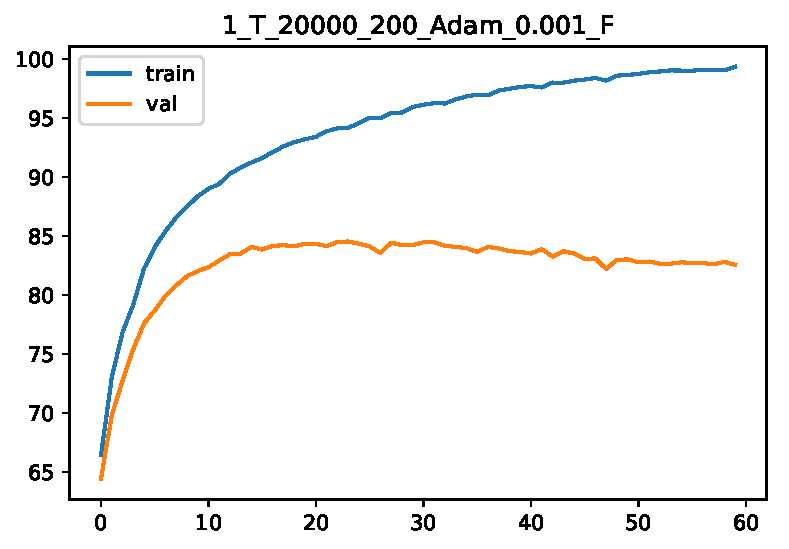
\includegraphics[width = 3cm]{1_T_20000_200_Adam_0001_F.pdf}
}	
\subfloat[(5000,500)]{
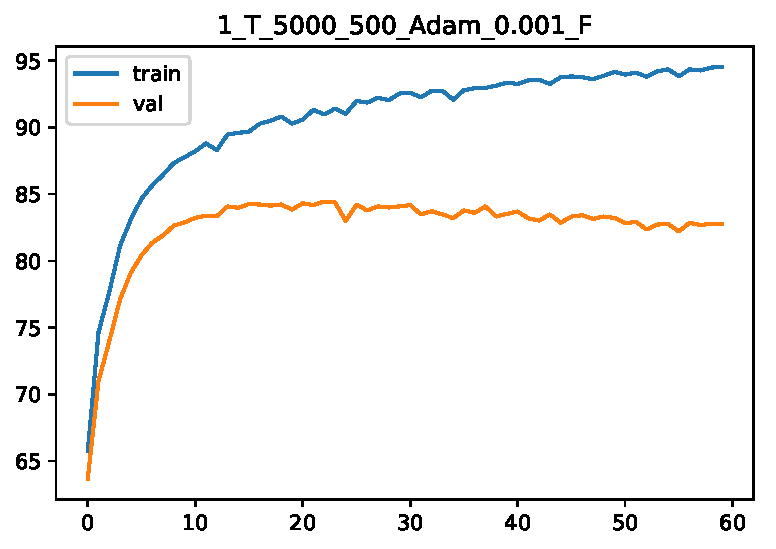
\includegraphics[width = 3cm]{1_T_5000_500_Adam_0001_F.pdf}
}	
\subfloat[(10000,500)]{
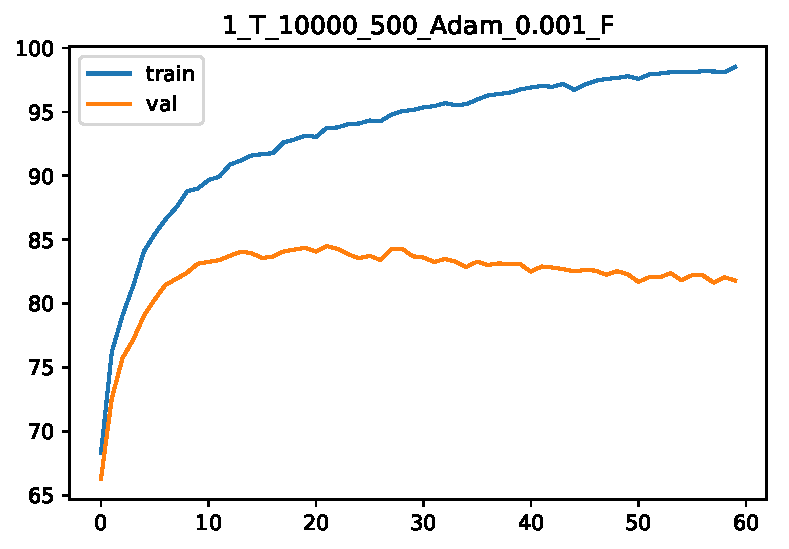
\includegraphics[width = 3cm]{1_T_10000_500_Adam_0001_F.pdf}
}	
\subfloat[(20000,500)]{
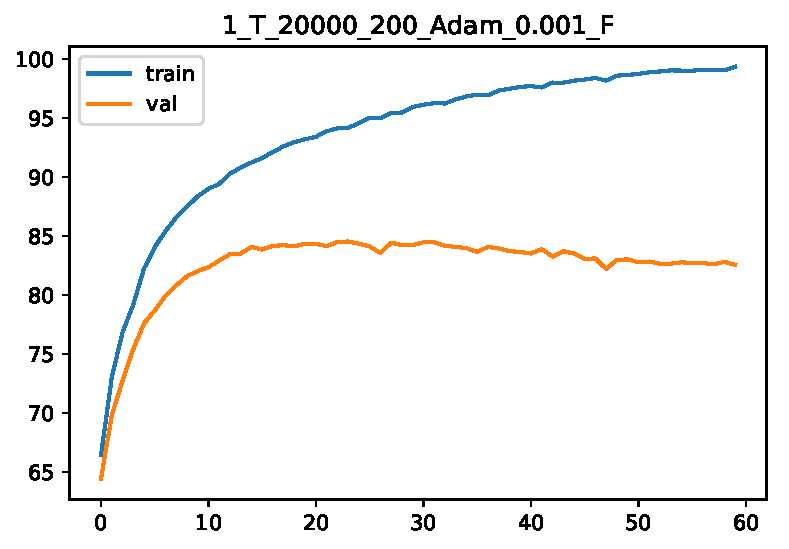
\includegraphics[width = 3cm]{1_T_20000_200_Adam_0001_F.pdf}
}	
\caption{\label{fig:vocab_emd}Vary Vocabulary Size and Embedding Size,  and Fix the Others Learning Curves.}
\end{figure}

We find the best vocab\_size and emd\_size are 5000,200. We plot the 9 learning curves in Figure \ref{fig:vocab_emd}.

 
\subsection{Vary Ngram, and Fix the Others}
We use the previously tuned best vocab\_size = 5000 and emd\_size = 200. We keep the optimization hyperparameters unchanged and vary n-grams strategy. The results are shown in Table \ref{tab: ngram}.
\begin{table}[!ht]
\centering
\begin{tabular}{|c|c|c|c|c|c|c|c|}
\hline
n & 1 &\multicolumn{2}{|c|}{2} & \multicolumn{2}{|c|}{3} & \multicolumn{2}{|c|}{4}\\ \hline
all\_gram & doesn't matter & True & False & True & False & True & False \\ \hline
Accuracy & 83.34 & 83.48 & 83.82 & 83.14 & 83.4 & 83.12 & 82.48\\ \hline
\end{tabular}
\caption{\label{tab: ngram}Accuracy on Validation Set When We Vary Ngram, and Fix the Others.}
\end{table}
The best configuration is 2-gram only without unigram with accuracy 83.82 on Validation Set.
\begin{figure}[!ht]
\centering
\subfloat[(1,T)]{
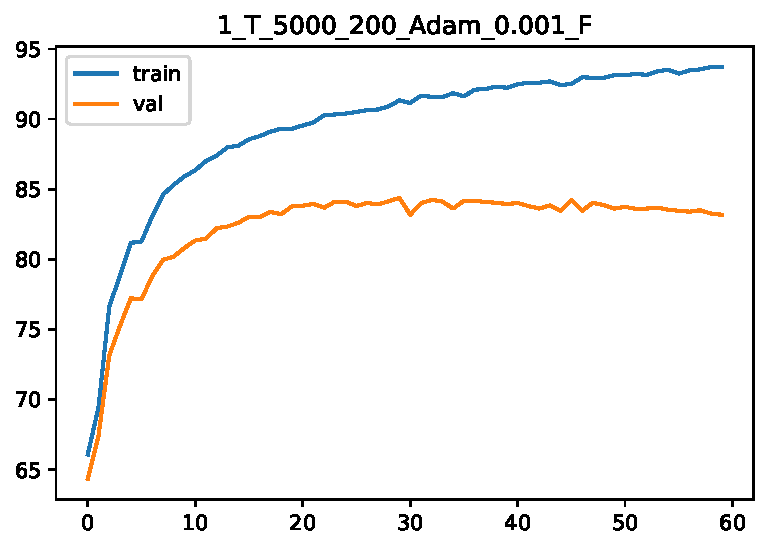
\includegraphics[width = 3cm]{1_T_5000_200_Adam_0001_F.pdf}
}
\subfloat[(2,T)]{
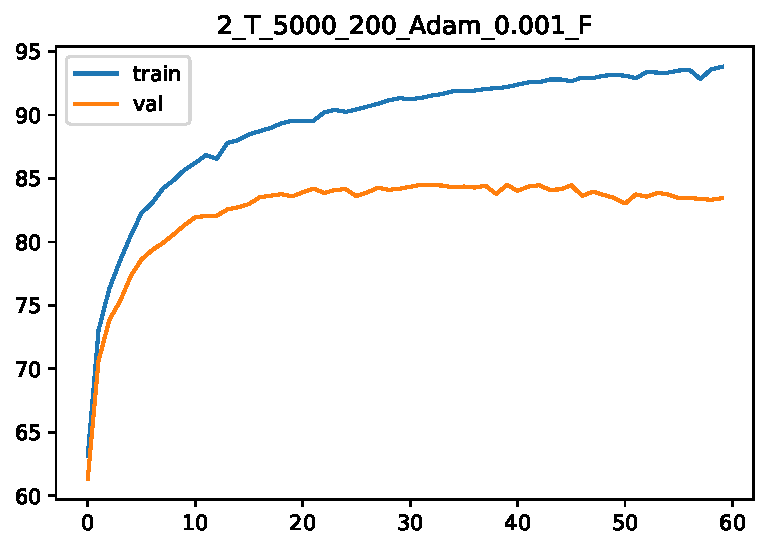
\includegraphics[width = 3cm]{2_T_5000_200_Adam_0001_F.pdf}
}	
\subfloat[(2,F)]{
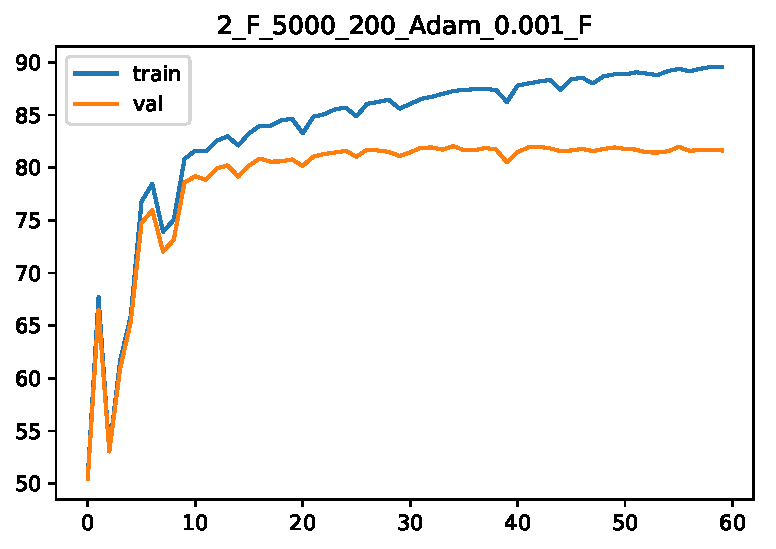
\includegraphics[width = 3cm]{2_F_5000_200_Adam_0001_F.pdf}
}	
\subfloat[(3,T)]{
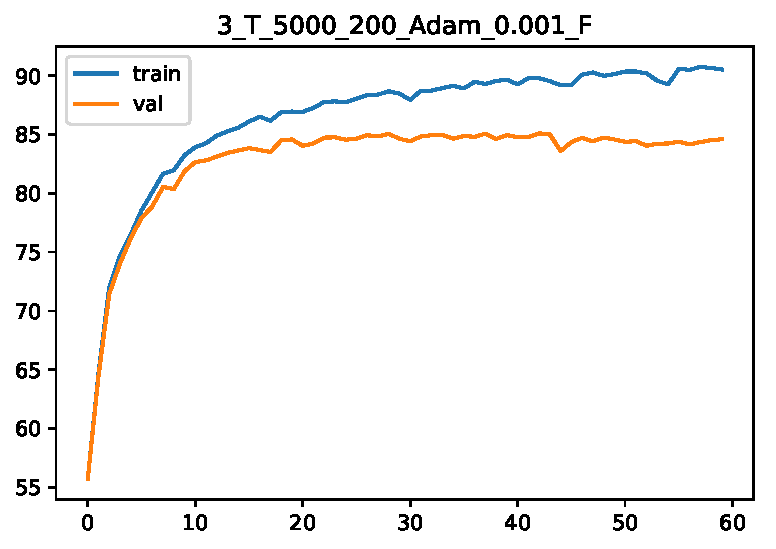
\includegraphics[width = 3cm]{3_T_5000_200_Adam_0001_F.pdf}
}		\\
\subfloat[(3,F)]{
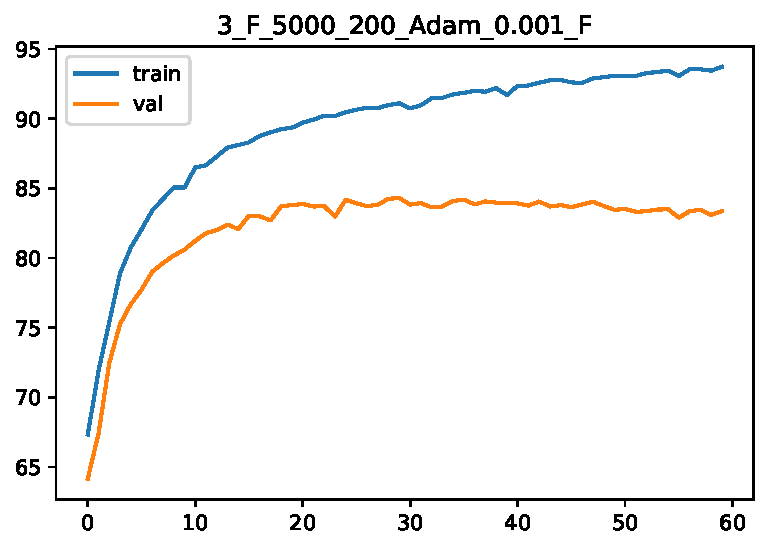
\includegraphics[width = 3cm]{3_F_5000_200_Adam_0001_F.pdf}
}		
\subfloat[(4,T)]{
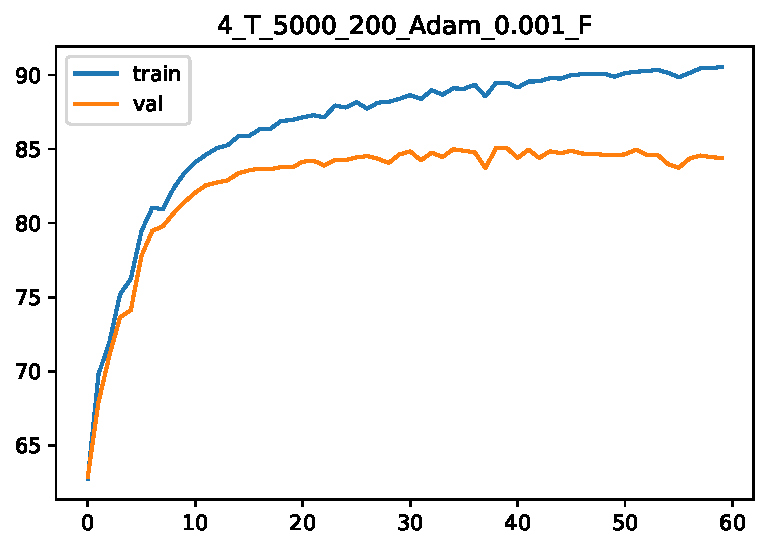
\includegraphics[width = 3cm]{4_T_5000_200_Adam_0001_F.pdf}
}	
\subfloat[(4,F)]{
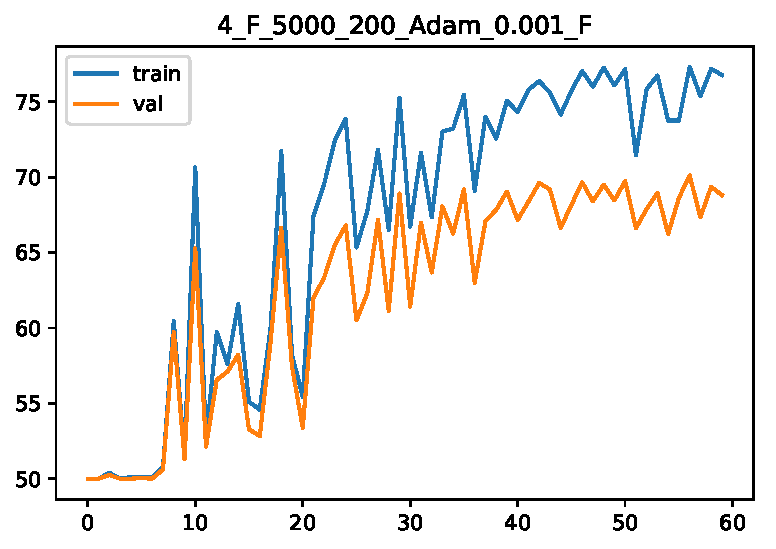
\includegraphics[width = 3cm]{4_F_5000_200_Adam_0001_F.pdf}
}	
\caption{\label{fig:ngram}Vary Ngram, and Fix the Others Learning Curves.}
\end{figure}
We plot the learning curves in Figure \ref{fig:ngram}.
\subsection{Vary Optimization and Fix the Others}
Finally we tune the optimization parameters. We fix n = 2, all\_ngram = False, vocab\_size =5000, emd\_size = 200 and vary optimization parameters.
\begin{table}[!ht]
\centering
\begin{tabular}{|c|c|c|c|c|c|c|c|c|c|c|c|c|}
\hline
Optimizer & \multicolumn{6}{|c|}{SGD} & \multicolumn{6}{|c|}{Adam} \\ \hline
lr\_decay & \multicolumn{3}{|c|}{True}& \multicolumn{3}{|c|}{False} &\multicolumn{3}{|c|}{True}& \multicolumn{3}{|c|}{False}\\ \hline
lr & 0.1 & 0.01 & 0.001 & 0.1 & 0.01 & 0.001 & 0.1 & 0.01 & 0.001 & 0.1 & 0.01 & 0.001\\ \hline
accuracy & 71.44 &64.94 &56.94 &71.08 &64.32 & 59.9&76.08& 80.08& 83.0 &80.0 & 80.36 & 83.24 \\ \hline
\end{tabular}
\caption{\label{tab: optim}Accuracy on Validation Set When We Vary Optimization and Fix the Others.}
\end{table}
We show the validation accuracies in Table \ref{tab: optim}. It turns out that our first choice of optimization hyperparameters are the best in the previous two sections. We are lucky! We plot the learning curves in Figure \ref{fig:optim}.
\begin{figure}[!ht]
\centering
\subfloat[(Adam,F,0.001)]{
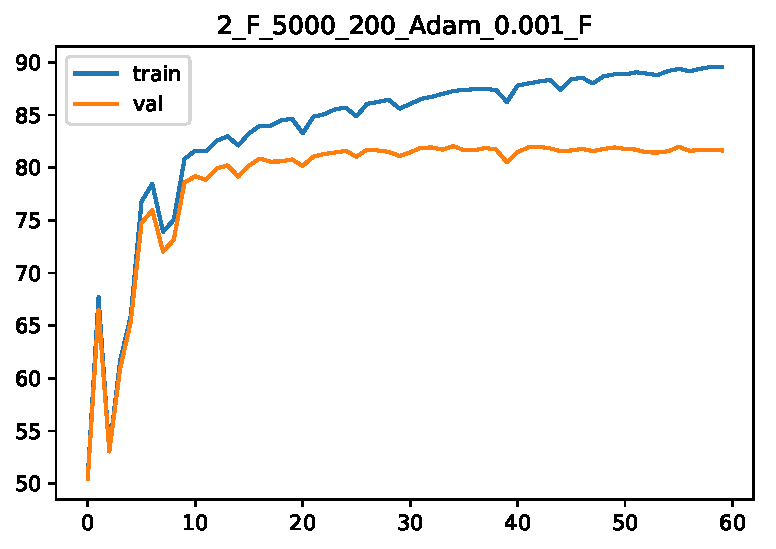
\includegraphics[width = 3cm]{2_F_5000_200_Adam_0001_F.pdf}
}
\subfloat[(Adam,T,0.001)]{
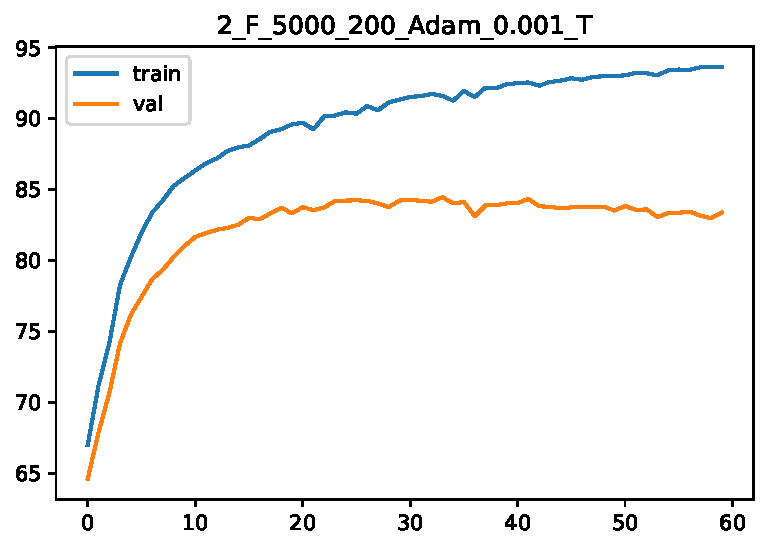
\includegraphics[width = 3cm]{2_F_5000_200_Adam_0001_T.pdf}
}	
\subfloat[(SGD,F,0.001)]{
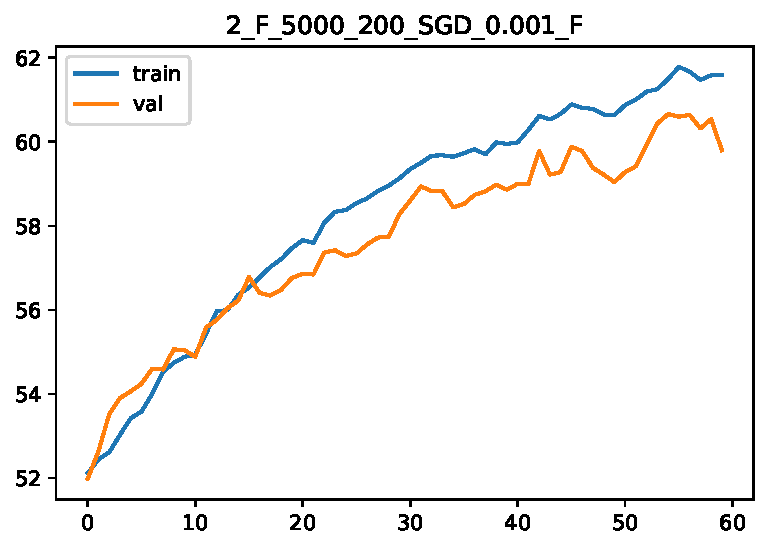
\includegraphics[width = 3cm]{2_F_5000_200_SGD_0001_F.pdf}
}
\subfloat[(SGD,T,0.001)]{
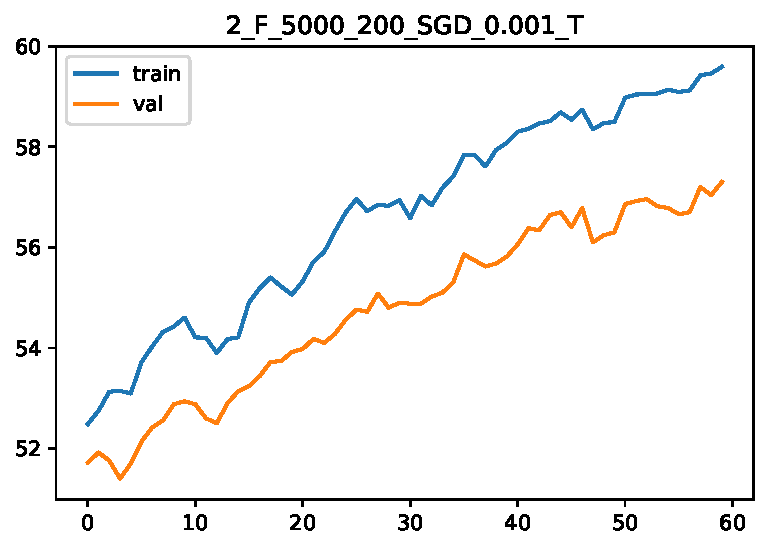
\includegraphics[width = 3cm]{2_F_5000_200_SGD_0001_T.pdf}
}		\\
\subfloat[(Adam,F,0.01)]{
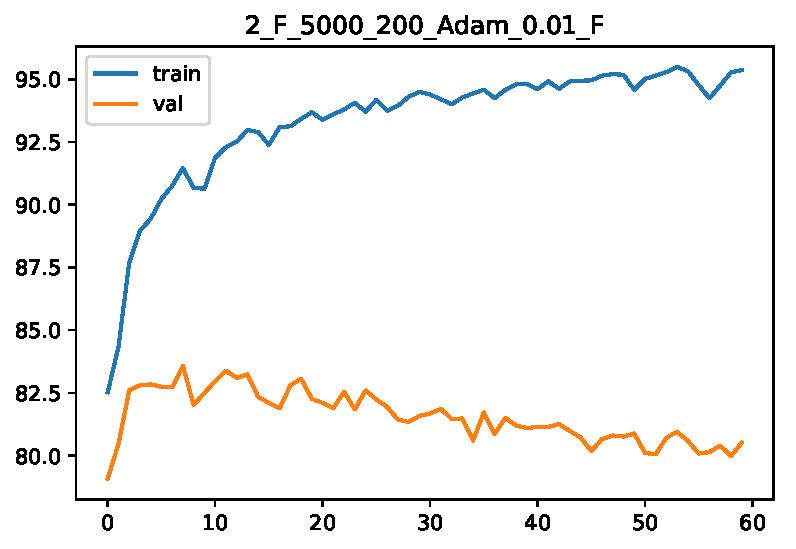
\includegraphics[width = 3cm]{2_F_5000_200_Adam_001_F.pdf}
}
\subfloat[(Adam,T,0.01)]{
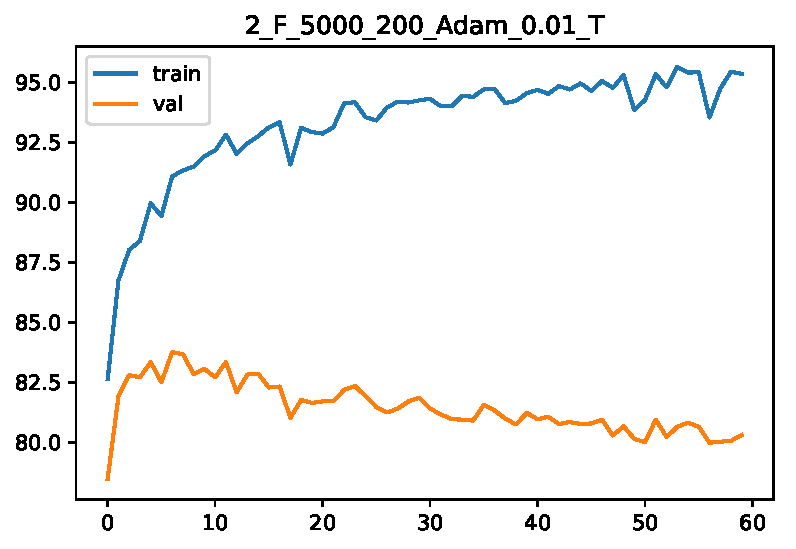
\includegraphics[width = 3cm]{2_F_5000_200_Adam_001_T.pdf}
}	
\subfloat[(SGD,F,0.01)]{
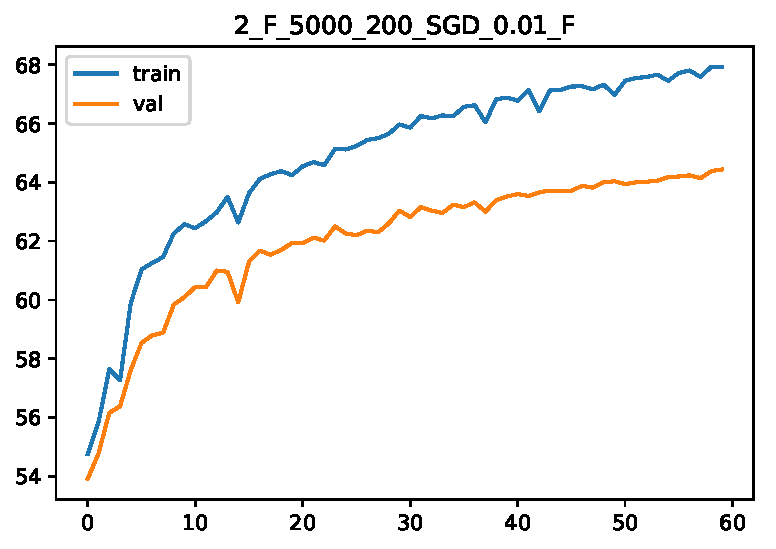
\includegraphics[width = 3cm]{2_F_5000_200_SGD_001_F.pdf}
}
\subfloat[(SGD,T,0.01)]{
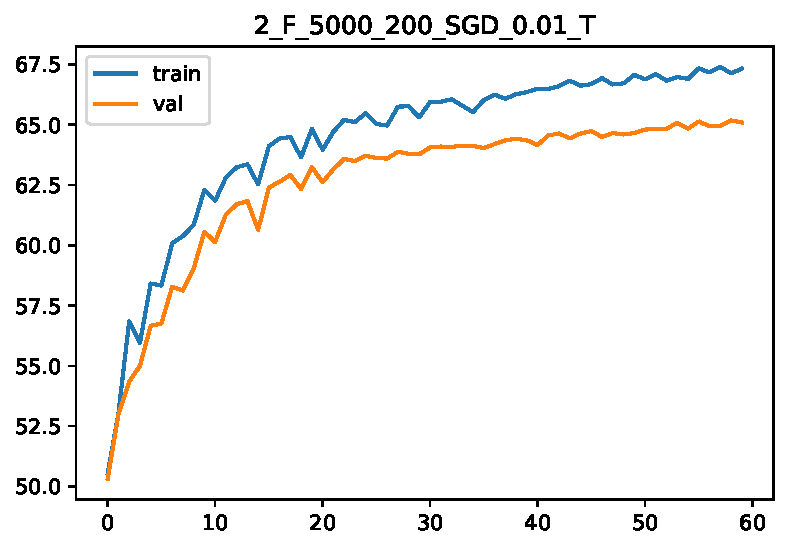
\includegraphics[width = 3cm]{2_F_5000_200_SGD_001_T.pdf}
}		\\
\subfloat[(Adam,F,0.1)]{
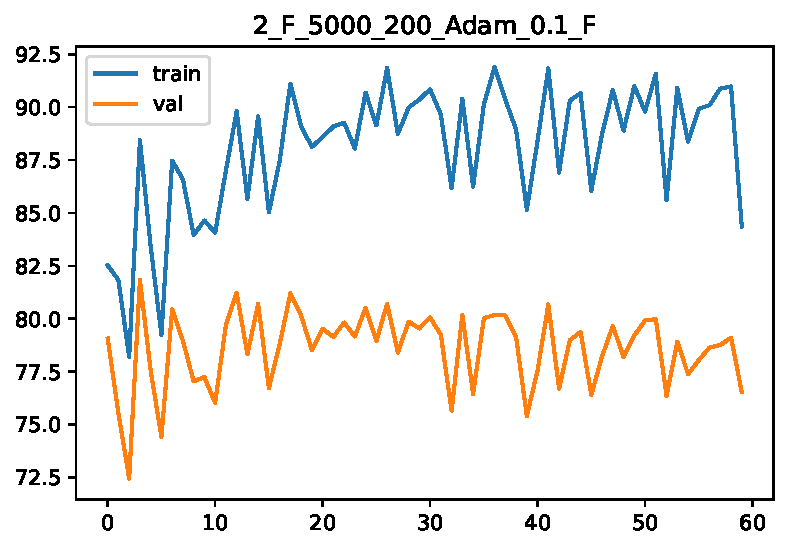
\includegraphics[width = 3cm]{2_F_5000_200_Adam_01_F.pdf}
}
\subfloat[(Adam,T,0.1)]{
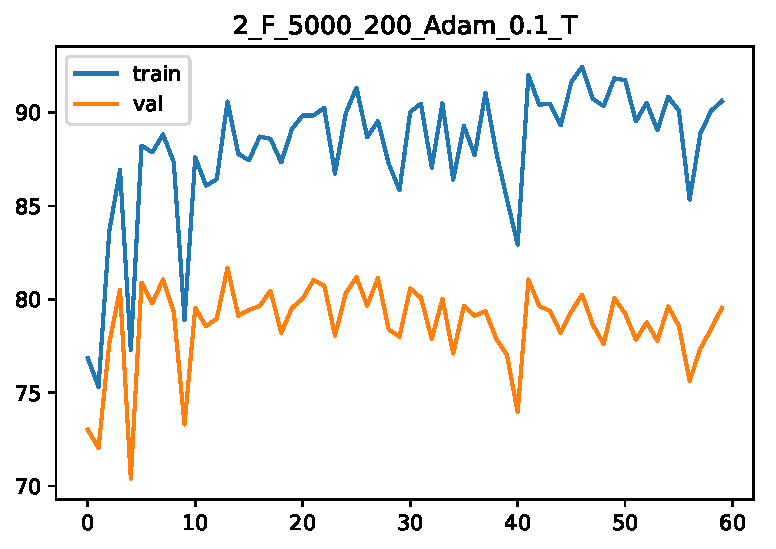
\includegraphics[width = 3cm]{2_F_5000_200_Adam_01_T.pdf}
}	
\subfloat[(SGD,F,0.1)]{
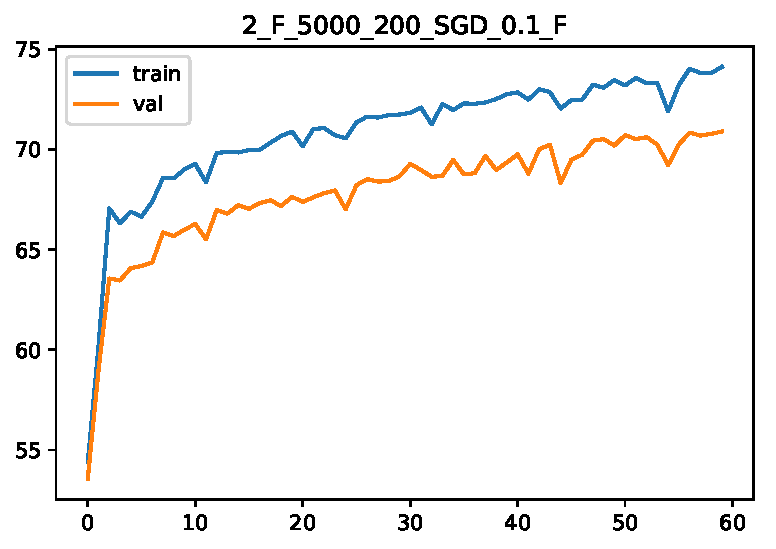
\includegraphics[width = 3cm]{2_F_5000_200_SGD_01_F.pdf}
}
\subfloat[(SGD,T,0.1)]{
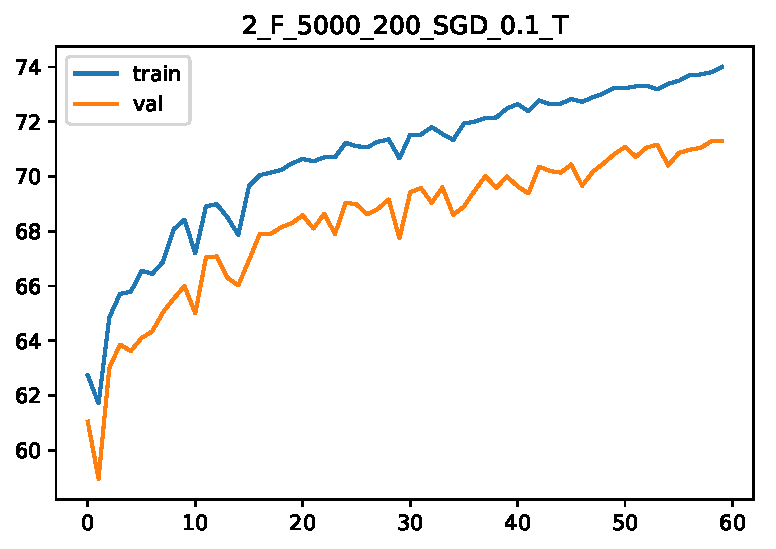
\includegraphics[width = 3cm]{2_F_5000_200_SGD_01_T.pdf}
}
\caption{\label{fig:optim}Vary Optimization and Fix the Others Learning Curves.}
\end{figure}
\subsection{List 3 Correct Predictions and 3 Incorrect Predictions}
Correct Predictions. They are all classified as negative.
\begin{itemize}
\item From what I understand, Mr. Bava abandoned this project before completion...AND RIGHTFULLY SO!!! If I were him I definitely would have made sure that EVERY copy was burned and if anybody in the future ever asked me about this film...IT NEVER HAPPENED \& IT NEVER EXISTED...end of story.<br /><br />Despite some great sets and good photography this is one horrible film...is it supposed to be scary? (not in the least) is it supposed to be funny?? (puh-leese) A total waste of time...and I really don't like to have to say that!!
\item Albert Pyun presents his vision of the lost city of Atlantis - and it's a vision so cluttered up with claustrophobic settings, weird costumes and noisy, "quirky" minor characters that one thing is for sure: you want to get the hell outta there as soon as possible (unfortunately, it will take you about 80 minutes). The "Alice in Wonderland"-like story is meandering and uninteresting, and there was probably no actress in the world who could have turned this into a good movie, though Kathy Ireland makes an appealing (annoying voice and all) attempt. (*1/2)
\item This started out as a good sketch comedy. The first few shows were very good and I was looking forward to a long run. What was really funny was the Mariah Carey imitation and the take off on Beverly Hills 90210 featuring the hair fight. The Delta Burke vs William Conrad heavy weight battle was also good. Unfortunately the following shows went downhill relatively quickly. The writing became uninspired and oh so predictable as if the show had acquired a cult following in it's young tenure. Nothing fresh was being offered and the recurring skits were boring. One example is the gun family (or whatever it was called) which became a weekly feature. This sketch was not all that funny to begin with let alone being a regular feature. An example of a quick promising start then a sudden fall.	
\end{itemize}
Incorrect Predictions. They should be negative but my model predicts them to be positive.
\begin{itemize}
\item The very first time I saw this I recoiled in HORROR at what was being presented as modern, liberated women.<br /><br />Sorry, but I cannot relate to whining idiots whose lives revolve around loveless sex and the acquisition of Gucci, Prada and Louis Vuitton labels. The troubling thing is that some may actually think this is how career women live in NYC. It's definitely not. These women are incredibly shallow and materialistic and as another reviewer said, they act like gold-digging hooches.<br /><br />This is not liberated womanhood and I'm glad it's gone. 0 stars and just plain AWFUL
\item I'm Mike Sedlak. I co-wrote the score for this movie. And proud of it. <br /><br />And I love all of the comments. Some have not gone far enough.<br /><br />The movie premiered in San Francisco in the summer of 1973. The theater was packed with friends and family. We all clapped.<br /><br />Five days latter, it was pulled from all of the screens in the Bay Area.<br /><br />If anyone is interested hearing some of scene by scene details, which might make the movie even more enjoyable, please let me know.<br /><br />We could start with the shot where Gideon Blake throws the toilet plunger to distract one of the evil henchmen guarding the radio transmitter on the deck of Bud's house. <br /><br />Or how Gideon diffused the bomb in the original version.<br /><br />Didn't help. It still bombed.<br /><br />Bring it on.
\item I know that this show gave a lot of liberation to women in the late '90s and early 2000s, but come on! You have a whiner, a buzz kill, and an over-analyzer. This show really made women look bad. I cannot STAND Carrie's analyzing every little thing on this show and that's what really killed it for me. Also, Charlotte's whining about her nonexistent predicaments made my ears hurt and Miranda's cynicism was a complete buzz kill. I mean, can't she just be happy? Samantha was the only cool one on the show and the only one worth watching. There was also a good episode when Nathan Lane was on the show, but that was the only one worth watching--the rest of them were pretty much the same. The humor was drier than a bucket of sand, and not very interesting plot line. All in all, not a very good show and I'm glad it's over.	
\end{itemize}

\section{Extra Points}
\subsection{Extra Hyperparamter Search}
We notice there is an extra hyperparameter in the code. That is MAX\_SENTENCE\_LENGTH. We choose three different values 150,200, and 250. We keep the other hyperparameters to be the optimal one we get in the previous section. Pleas see the code in $\texttt{hw1.ipynb}$ for reference. When we increase the MAX\_SENTENCE\_LENGTH from 150 ,200 to 250. The validation accuracy rises from 81.46, 83.3 tp 84.1. So the MAX\_SENTENCE\_LENGTH is an important hyperparameter. And the test accuracy for MAX\_SENTENCE\_LENGTH=250 model is 85.132.

There is another hyperparameter number of the epochs.  We try number of epochs 5 instead of 10 . We get 84.54 on validation set and 85.916 on test set. This is an improvement! So the final \textbf{test score} in this homework is \textbf{85.132}. 
\subsection{Train 1-10 rating}
Instead of training negative and positive reviews, we could also train a 1-10 rating. In order to do so, we train a 10 class classifier. Pleas see the code in $\texttt{hw1.ipynb}$ for reference. I use the previous configuration from binary classification. It turns out that the accuracy is very low. I think the reason is that the model is two simple for 10-class classification. The validation accuracy is the 32.12. and the test accuracy is 34.4.
\end{document}









